\documentclass{article}
\usepackage[UTF8]{ctex}
\usepackage{picinpar,graphicx}
\usepackage{float}
\usepackage{geometry}
\usepackage{indentfirst}
\usepackage{listings} 
\usepackage{xcolor}
\geometry{left=2.0cm,right=2.0cm,top=2.0cm,bottom=2.0cm}

\title{Java零基础从入门到就业}
\author{Miels Herro}
\date{}

\begin{document}
\maketitle

\section{初识Java}	
	\subsection{计算机语言的发展历史}
	第一代:机器语言:机器语言是机器能直接识别的程序语言或指令代码,无需经过翻译,每一操作码在计算机内部都有相应的电路来完成它,或指不经翻译即可为机器直接理解和接受的程序语言或指令代码。
	
	第二代:汇编语言:发明了一些助记符,用助记符代替机器指令的操作码,用地址符号或标号代替指令或操作数的地址。
	
	第三代:高级语言(隐藏了人与计算机之间的障碍)
	
	不要争什么语言是最好的语言,只有在一定领域内最适合的语言。
	
	整个高级语言一部分是面向过程的,一部分是面向对象的(Java属于后者,后面会进一步理解)
	
	\subsection{Java简史}
	James Gosling发明
	
	1991年,SUN公司的Green项目Oak;1995年,推出Java测试版……2009年,甲骨文(Oracle)收购SUN
	
	Oracle公司提出“小步迭代,快速奔跑”的理念,推出来之后让用户们测(本次课程使用JDK8,因为8、11、17才是JDK长期维护的版本;并且用最新的版本的话,可能有些软件不支持;还有就是8和9的目录结构会有所不同)
	
	\begin{figure}[ht]
		\centering
		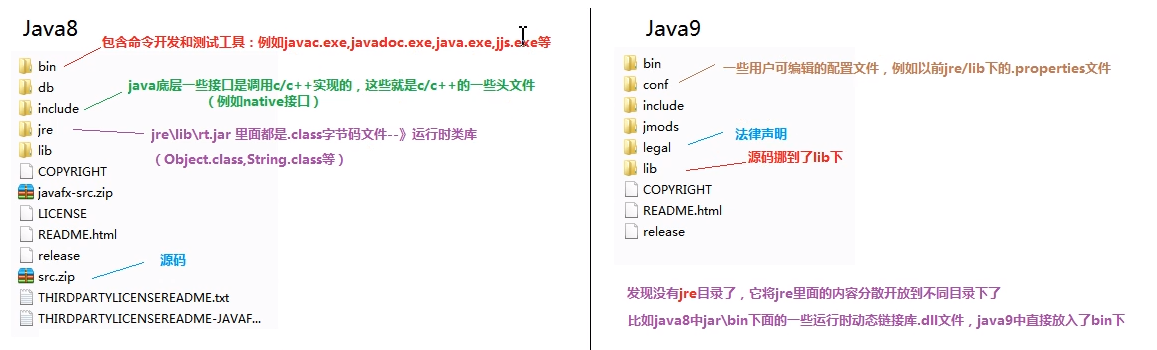
\includegraphics[width=120mm]{1.png}
		\caption{8和9的目录变化}
		\label{fig:label}
	\end{figure}

	\subsection{Java体系结构}
	JavaSE(Java Standard Editon, aka J2SE),定位在个人计算机上的应用。学会了最基础的知识,可以做桌面级的应用(坦克大战,超级玛丽,五子棋……),但是做不了网站,这就需要学习EE部分了
	
	JavaEE(Java Enterprise Editon),定位在服务器端的应用。作为JavaSE的扩展,增加了用于服务器开发的库。
	
	JavaME(Java Micro Editon),以前玩的手机上的小游戏可能就是用ME编写的。
	
	之所以应用场合不一样,本质是因为底层语言包含的类就不一样(现在先不涉及“类”的讲述)
	
	\begin{figure}[ht]
	\centering
	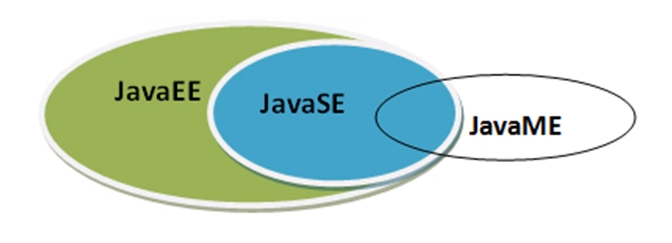
\includegraphics[height=40mm]{2.png}
	\caption{Java体系}
	\label{fig:label}
	\end{figure}	
	
	\subsection{Java核心机制1——垃圾收集机制}
	任何程序运行都是会有垃圾出现的,程序运行时,会在内存中(给变量、对象等)开辟空间,使用完毕后就需要清除掉,相当于“释放内存”的过程。
	
	C++程序中的释放内存需要手动进行操作,清多少,还多少都要考虑。
	
	Java底层有一个垃圾收集器(Garbage Collector, GC),不用人管,自动释放,同时程序员无法精确控制和干预,但是提高了内存空间的利用效率,提高了编程人员的效率,很大程度上减少了因为没有释放空间而导致的内存泄漏。
	
	更高级的问题:
	
	1、GC有几种呢?
	
	2、GC底层原理剖析?
	
	3、GC算法是什么呀?能不能有一定的优化呢?

	\subsection{Java核心机制2——跨平台原理}
	
	任何语言在写完代码之后,都会产生一个文件,假设这里所写内容为“HelloWorld”,则若用html语言编写,则生成\ HelloWorld.html\ 或\ HelloWorld.htm\ 文件,若用C语言编写,则生成\ HelloWorld.c\ 文件,若用python编写,则生成\ HelloWorld.py\ 文件,用Java编写则生成\ HelloWorld.java\ 文件(源文件)。
	
	源文件内一定是实现了一个案例(比如进行了自我介绍),文件是死的,最终要把文件在对应的平台上运行。假设现在系统1是Windows系统,.java\ 源文件不能在系统上直接运行,要经历一个过程:.java源文件转变为.class字节码文件(这一过程叫做“编译”)
	
	.class字节码文件不能直接被Windows系统识别(可类比为中国人去了美国,需要一个翻译),在系统1\ Windows平台上对应有程序叫“虚拟机(JVM)”可以把.class文件翻译(这一过程叫做“执行”或者“翻译”)

	虚拟机的作用:翻译官(将.class字节码文件翻译为当前平台认识的可执行文件的格式)
	
	编译需要的命令是“javac.exe”;
	
	执行需要的命令是“java.exe”。
	
	(在执行的时候,表面上调用的是java.exe,实际上会动态调用JVM,实际真正起到执行作用的是虚拟机JVM。虚拟机JVM将.class字节码文件逐行解释为当前系统认识的可执行文件,所以Java是一种“解释型语言”)
	
	如果想要把.class字节码文件在系统2\ Linux平台上运行,则还需要另外的对应的虚拟机JVM。
	
	如果想要把.class字节码文件在系统3\ MacOS平台上运行,则还需要另外的对应的虚拟机JVM。
	
	(就像是中国人出国玩,去美国要带一个翻译官,去韩国、日本同样需要翻译官)
	
	这也就是所谓的“一次编译,到处运行(Write Once, Run Everywhere)”,跨平台原理也即如此。
	
	上述的javac.exe和java.exe都在JDK软件中。
	
	\begin{figure}[ht]
		\centering
		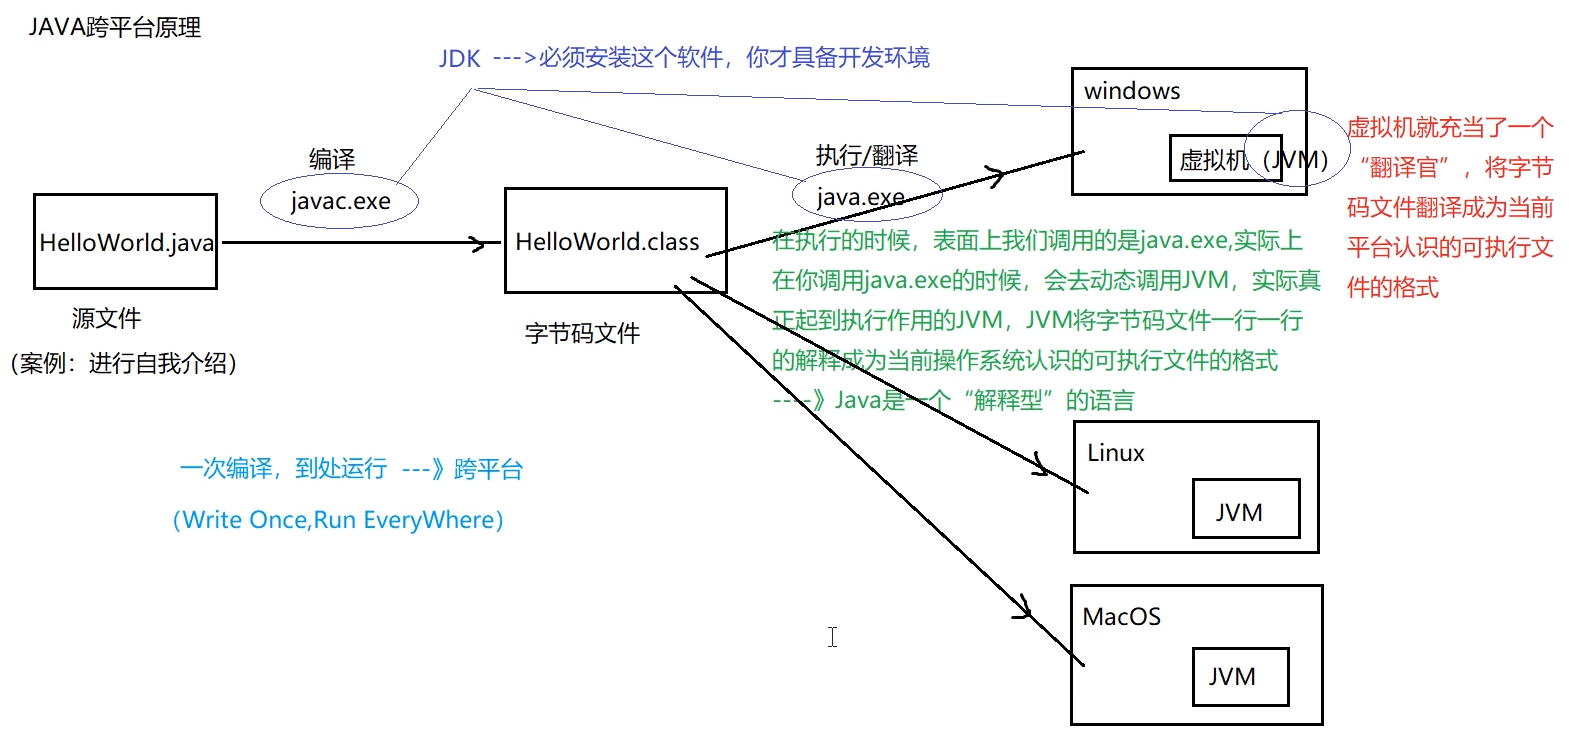
\includegraphics[width=180mm]{3.png}
		\caption{Java跨平台原理}
		\label{fig:label}
	\end{figure}	

	\subsection{横向对比——C语言的跨平台原理}
	
	假设内容相同,所用语言改为C语言,则最初会生成HelloWorld.c源文件。.c源文件经过Windows专用编译器之后产生可执行文件,可执行文件再转入Windows平台运行,并且若将此可执行文件转入Linux平台,不可以运行,所以编译器是与平台相关的,而且所产生的可执行文件也是和平台相关的。
	
	若HelloWorld.c文件想要在Linux平台上运行,则需要Linux专用编译器编译产生Linux平台对应的可执行文件,再转入Linux平台后可以才可以运行。
	
		\begin{figure}[ht]
		\centering
		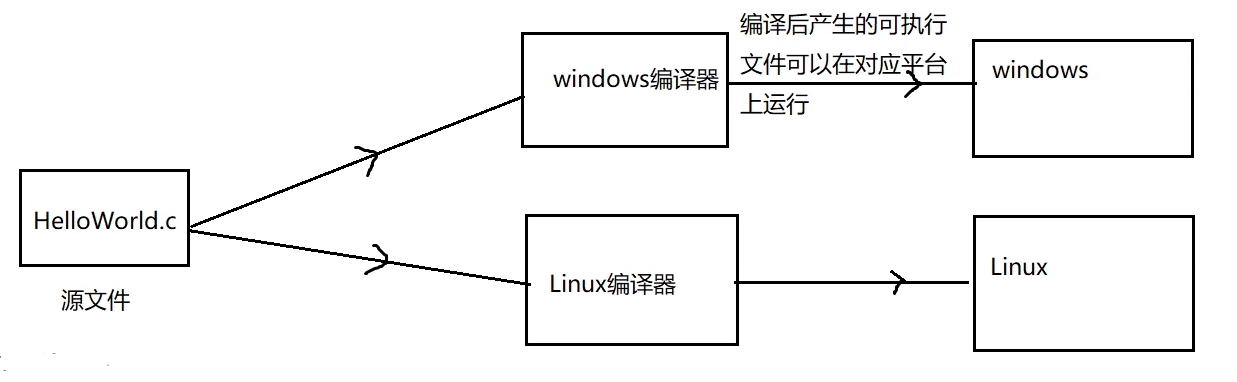
\includegraphics[width=120mm]{4.png}
		\caption{C语言跨平台原理}
		\label{fig:label}
	\end{figure}
	
	C语言跨平台和Java跨平台的区别:
	
	\setlength{\parindent}{4em}
	(1)Java的字节码文件是与平台无关的,同一个字节码文件可以到不同的平台上去运行
	
	(2)C语言针对不同的平台有不同的编译器
	
	\setlength{\parindent}{6em}
	(编译器与平台相关,编译后的可执行文件也是与平台相关的)
	
	\setlength{\parindent}{2em}
	C语言是不是跨平台的呢?
	
	答:此处的跨平台指的是——编译后的文件是否跨平台。从此角度来看,C语言不是跨平台的(C语言源文件是可以跨平台的,故常在网上被人宣传为“C语言是跨平台语言”)
	
	\ 
	
	C语言效率高还是Java效率高呢?
	
	答:C语言的效率高。因为C语言源文件编译后的可执行文件可以直接在平台上运行,而Java还需要虚拟机JVM逐行解释翻译为平台所认识的语言。
	
	\subsection{常用DOS命令}

	DOS和Windows最大的区别是:Windows有很好的图形操作界面,而DOS系统下的类似操作都需要通过代码操作(Windows保留了此操作系统,通过Win+R,再输入cmd进入“控制命令台”)
	
	命令“D:”\ 可从默认C盘切换进D盘(大小写不做区分);
	
	命令“dir”\ 可显示当前盘内详细信息;
	
	命令“cd Doc”\ 可进入Doc文件夹(.\ 代表当前目录,..\ 代表上层目录);
	
	命令“cd..”\ 可返回上一层目录D盘;
	
	命令“cls”\ 可清屏(只是障眼法,点击上下箭头可以切换历史命令)
	
	命令“Tab”\ 可自动补全目标文件夹名(进入Doc文件夹之后,只输入J,单击Tab跳出JavaCode,再次单击跳出Job,再次单击跳出JRCODE)
	
	命令“md a”\ 可创建目录a;

	命令“rd a”\ 可删除目录a;
	
	命令“copy demo.txt a\ 1.txt”\ 可复制dome.txt文件到当前文件夹下的a文件夹下的1.txt文件内;
	
	命令“del demo.txt”\ 可删除文件demo.txt;
	
	命令“del a”\ 可删除目录a内部的文件,但文件夹仍然存在;
	
	\subsection{Notepad++相关}
	
	打开Notepad++的方式:
	
		\setlength{\parindent}{4em}
	(1)双击桌面快捷方式
	
	(2)控制命令台方式:Win+R输入cmd→进入Notepad++所在文件夹→输入Nptepad++→回车
	
	(3)控制命令台下在D盘内执行Notepad++(一开始会报错,就需要配置系统的环境变量)
	
	(进入环境系统变量,选择Path,加入Notepad++所在路径)
	
	\begin{figure}[ht]
		\centering
		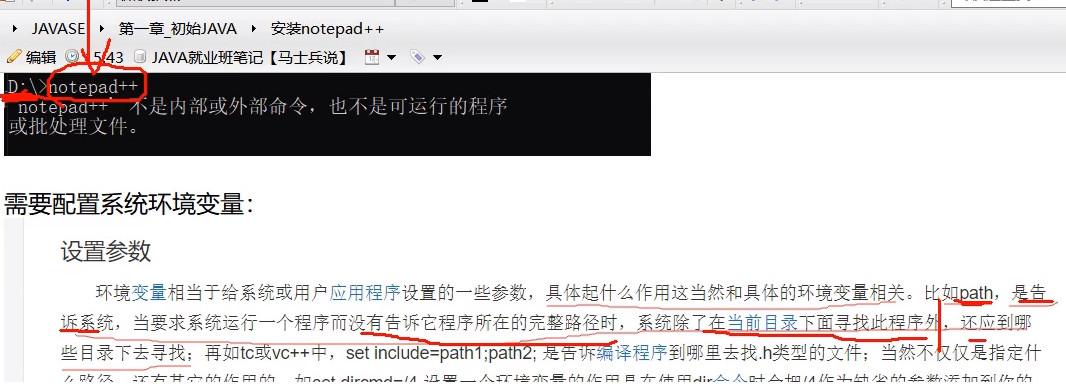
\includegraphics[height=50mm]{5.png}
		\caption{配置环境变量}
		\label{fig:label}
	\end{figure}
	
	\ 
	
	\ 
	
	\ 
	
	\ 
	
	\ 
	
	\subsection{第一段程序}
	
	public class HelloWorld{
		
		\setlength{\parindent}{6em}public static void main(String[] args){
		
			\setlength{\parindent}{8em}System.out.println("hi 这是一段Java程序。。。")
	
		}
		
	}
	
	\begin{figure}[ht]
		\centering
		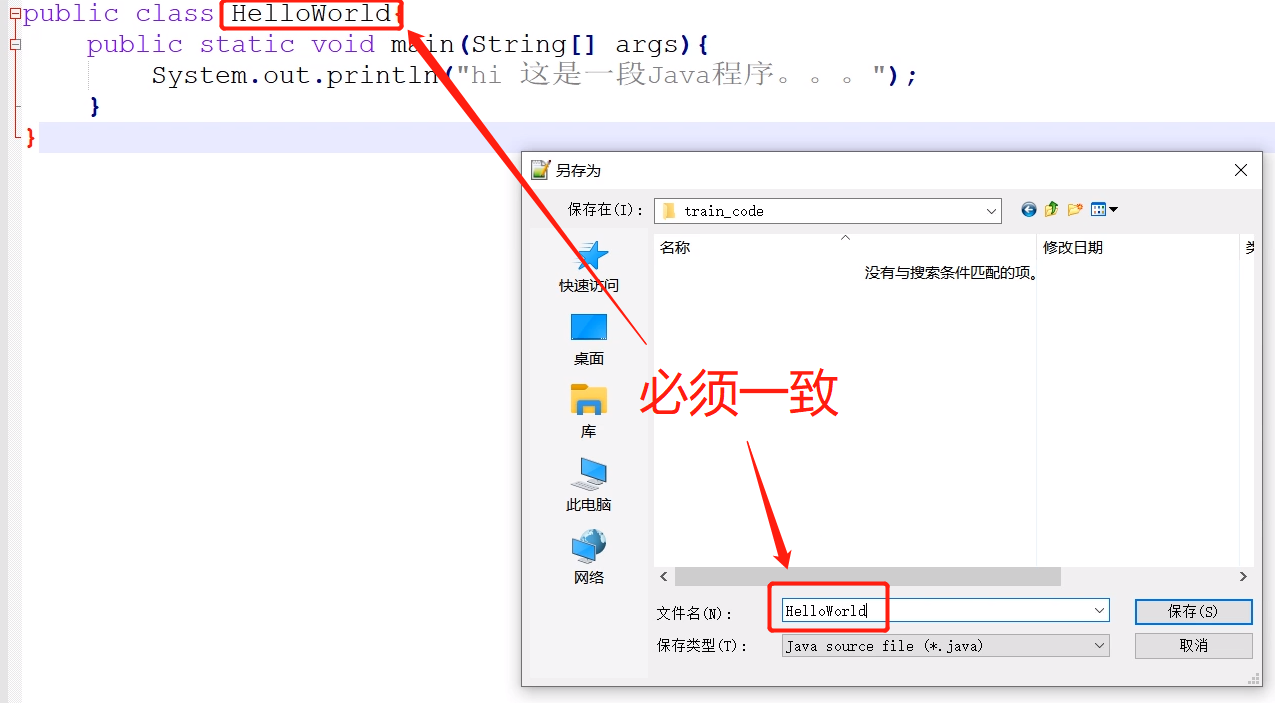
\includegraphics[height=40mm]{6.png}
		\caption{编写代码及保存}
		\label{fig:label}
	\end{figure}
	
	\setlength{\parindent}{2em}
	产生文件“HelloWorld.java”源文件(接下来需要通过javac.exe编译变成.class字节码文件)
	
	\begin{figure}[hb]
		\centering
		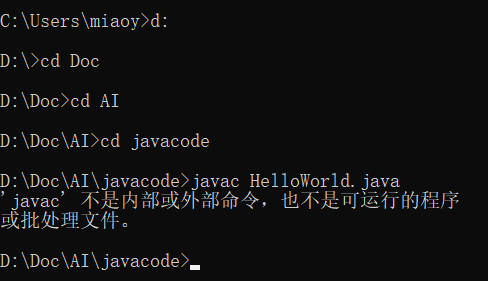
\includegraphics[height=50mm]{7.png}
		\caption{javac.exe编译.java源文件出错}
		\label{fig:label}
	\end{figure}
	
	\ 
	
	\ 
	
	\ 
	
	分析原因:
	
	\setlength{\parindent}{4em}
	HelloWorld.java源文件确实位于javacode文件夹内,故不是由文件位置放置错误所引起;
	
	javac.exe命令在D:$\backslash$Softwares$\backslash$JDK$\backslash$bin路径下放置;
	
	综上所述,“javacode路径下找不到javac.exe”\setlength{\parindent}{4em}是出错的原因。
	
	\begin{figure}[ht]
	\centering
	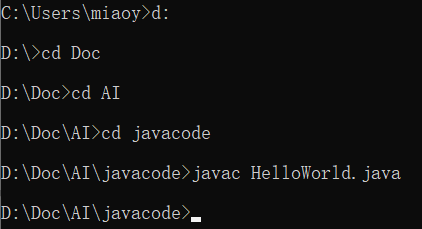
\includegraphics[height=40mm]{8.png}
	\caption{修改环境变量之后成功运行}
	\label{fig:label}
	\end{figure}	
	
	\setlength{\parindent}{2em}
	检查D:$\backslash$Doc$\backslash$AI$\backslash$javacode文件夹后,发现确实生成了HelloWorld.class字节码文件
	
	接下来直接执行.class字节码文件,输入如下:
	
	\begin{figure}[ht]
		\centering
		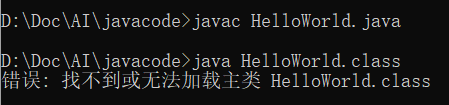
\includegraphics[width=80mm]{9.png}
		\caption{尝试运行.class字节码文件报错}
		\label{fig:label}
	\end{figure}	
	
	分析原因:
	
	\setlength{\parindent}{4em}
	按照当前输入,程序运行的是HelloWorld.class.class文件,但是文件夹中并没有这个文件;
	
	因此要输入"java HelloWorld"。
	
	\begin{figure}[ht]
		\centering
		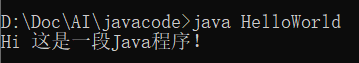
\includegraphics[width=80mm]{10.png}
		\caption{成功运行.class字节码文件运行结果}
		\label{fig:label}
	\end{figure}
	
	\subsection{程序常见问题}
	
	\setlength{\parindent}{2em}
	1、单词拼写错误;
	
	2、程序中的class类名和.java源文件的名字必须一致;
	
	3、所有标点必须是英文状态下的;
	
		\setlength{\parindent}{5em}【】(){}!;:“”?
	
\ \ 	[]\ \ \ ()\ {}\ !\ ;\ :\ ""\ \ ?
	
		\setlength{\parindent}{2em}
		4、成对编程
		
		5、注意缩进:只要遇到{}就缩进
		
		\ 
		
		\setlength{\parindent}{4em}缩进:tab
		
		向前缩进:shift+tab
		
		\setlength{\parindent}{2em}
		6、编译:javac HelloWorld.java
		
		7、执行:java HelloWorld
		
		8、Java对大小写非常敏感
		
		9、初期写代码的时候就当作有一个固定格式:
		
		\begin{lstlisting}
		public class HelloWorld{
			public static void main(String[] args){
			XXXXXXX
			}
		}
		\end{lstlisting}
		
		(HelloWorld\ 和\ args可以随便起名字,其余部分必须严格按照这个来)
		
		10、一个源文件中只能由有一个public class,.java源文件的名字必须与public class名字一致

\begin{figure}[ht]
	\centering
	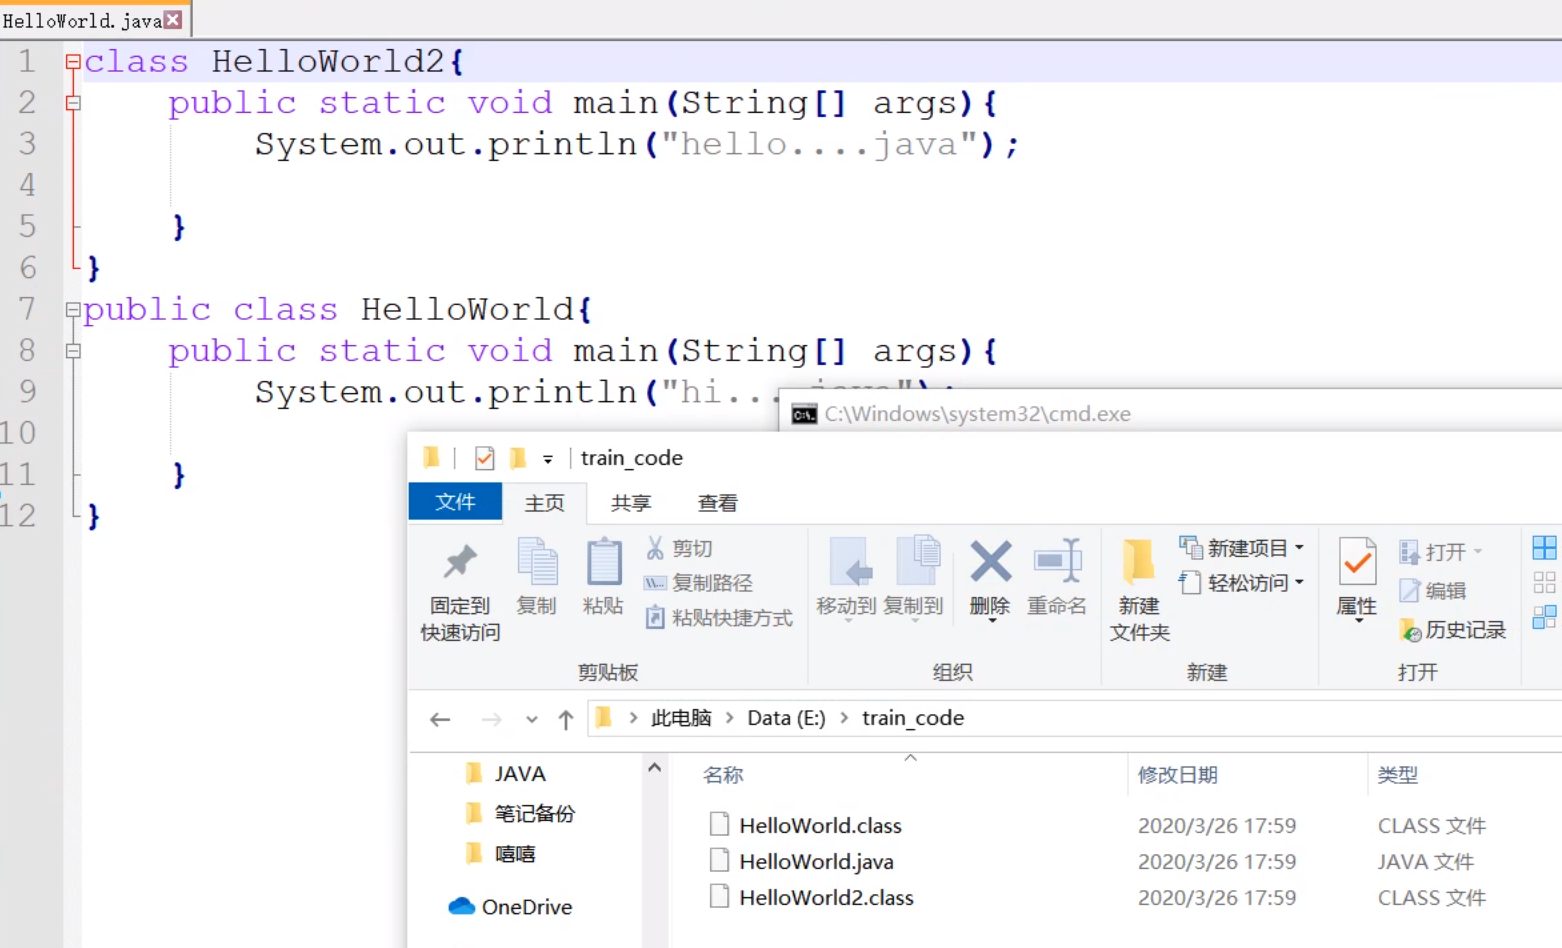
\includegraphics[width=80mm]{11.png}
	\caption{每个类产生各自的字节码文件}
	\label{fig:label}
\end{figure}			

		(执行不同的字节码文件会输出不同的结果,互相并不冲突)

		\subsection{编译方式}
		
		方式1:进入命令控制台,进入目标文件夹,javac HelloWorld.java进行编译;
		
		方式2:如图12;
\begin{figure}[ht]
	\centering
	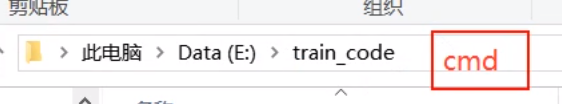
\includegraphics[width=60mm]{12.png}
	\caption{进入目标文件夹目录输入cmd,再输入javac HelloWorld.java进行编译}
	\label{fig:label}
\end{figure}		

		方式3:如图13;
		\begin{figure}[ht]
			\centering
			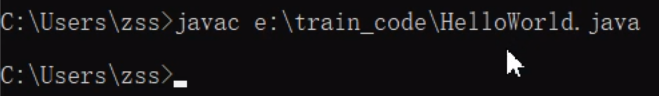
\includegraphics[width=60mm]{13.png}
			\caption{进入命令控制台,输入javac D:$\backslash$Doc$\backslash$AI$\backslash$javacode$\backslash$HelloWorld.java进行编译}
			\label{fig:label}
		\end{figure}	
	
		方式4:在Notepad++中右键单击文件,选择“打开所在文件夹(命令行)”,输入javac HelloWorld.java
		
		\subsection{环境变量讲解}
		
		1、classpath:系统中本身就有一个环境变量叫classpath,只不过没有显式表达出来,如果人工配置classpath的路径之后,在执行.class字节码文件的时候,就会去配置的路径下去找对应的字节码文件。
		
		(classpath是专门针对java程序编写时执行.class字节码文件而设定的环境变量;只要配置了字节码文件得位置,今后在任何位置都可以执行.class字节码文件)
		
		2、JAVA\_ HOME环境变量:后续会使用tomcat软件,点击bin目录下的startup.bat文件会出现闪退问题;为了解决以上问题需要配置JAVA\_HOME环境变量,其变量值为jdk所在路径;
		
		然后在Path环境变量中就可以对JAVA\_HOME进行引入,方式为\%JAVA\_HOME\%
		
		\subsection{API(Application Programming  Interface)}
		
		API就是一个用来查看JAVA涉及技能点的电子文档
		
		\subsection{注释}
		
		单行注释://注释
		
		多行注释:/*
		
		\setlength{\parindent}{8em}注释
		
		\setlength{\parindent}{7em}*/
		
		\setlength{\parindent}{2em}文档注释:/**
		
		\setlength{\parindent}{8em}@author miaoyulu
		
		@version 1.0
		
		@param name 姓名
		
		@param age 年龄
		
		\setlength{\parindent}{7em}*/
		
		\setlength{\parindent}{2em}	注意:①编译后产生的字节码文件中不会有注释的内容;②提高代码可读性(职业习惯);③代码调试排错时非常有用;④一般文档注释可以:使用javadoc.exe对文档注释进行解析,生成一套以网页形式说明文档(点击index.html文件即可,命令如下图)
		
		\begin{figure}[ht]
			\centering
			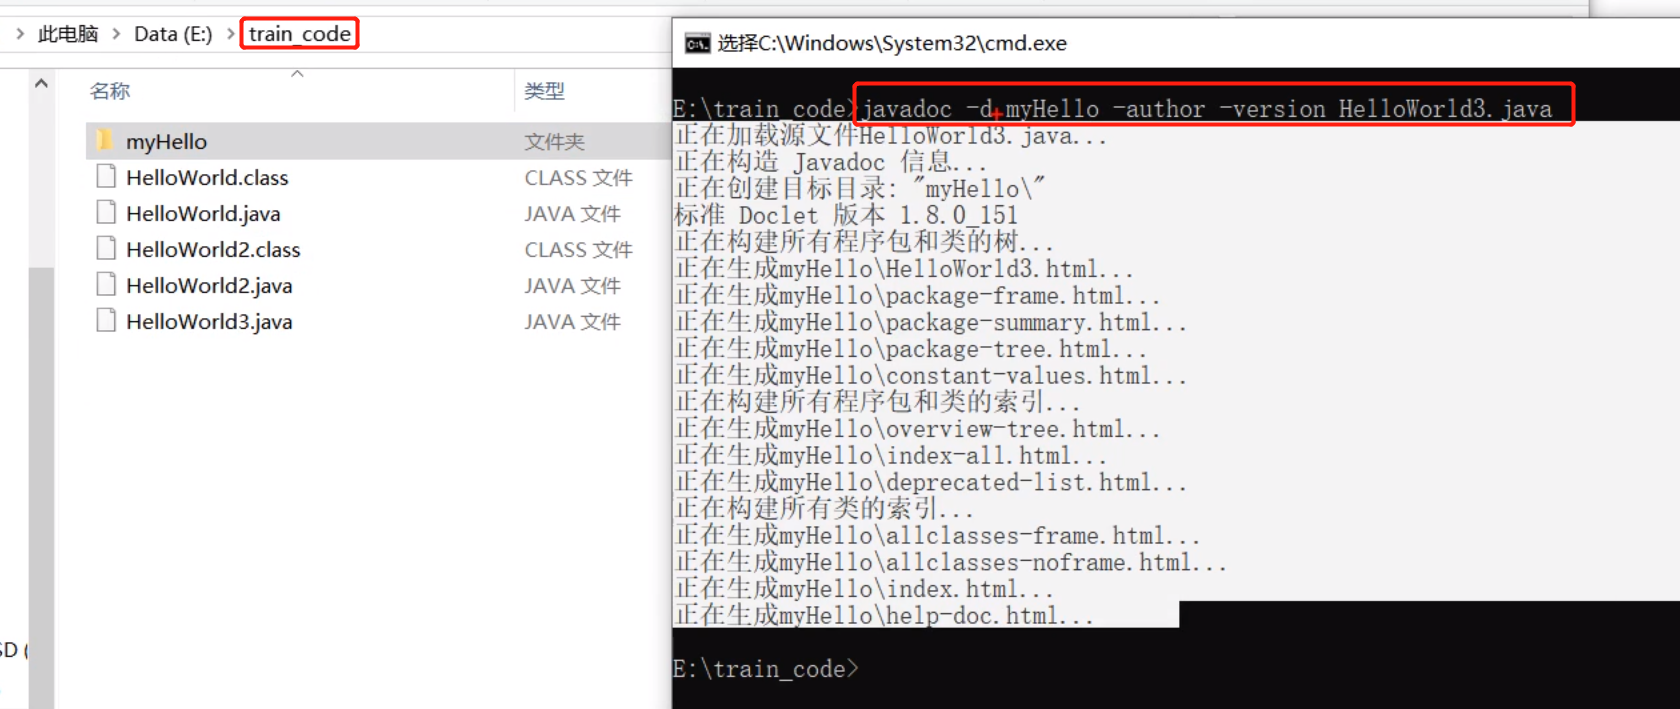
\includegraphics[width=100mm]{14.png}
			\caption{使用javadoc.exe对文档注释进行解析}
			\label{fig:label}
		\end{figure}
		
		\subsection{使用反编译工具}
		
		对于Java虚拟机来说,执行的是.class字节码文件,故而在合作时只分享.class字节码文件,而不分享.java源文件。如果我想要修改源文件,那就需要把.class字节码文件还原为.java源文件,这时就需要反编译工具。
		
		注意:反编译工具打开.class字节码文件后发现并没有注释,二次证明了注释不参与编译中;有一个引入,当前可以不理解;形参不重要,注重的是传输进去的实参。
		
		\subsection{本章最后一段代码}
		
		System.out.print("")输出内容后不换行;System.out.print("")输出后换行。
		
		只要代码改过就要重新编译。
		
		System.out.print("$\backslash$ n")输出内容后换行。
		
		转义字符$\backslash$t的空格数和前一个字符加起来是一个制表符,即8位。
		
		\subsection{拓展面试题:JDK,JRE,JVM的区别}
		
		JDK(开发工具包)包含JRE(运行环境)包含JVM(虚拟机)
		
		开发人员装JDK即可,运行人员装JRE即可。
		
		D:$\backslash$Softwares$\backslash$JDK$\backslash$lib$\backslash$文件路径下的dt.jar和tools.jar是Java最核心的两个包。输入javac命令时并不是去JDK的bin目录下去找javac.exe,而是去JDK$\backslash$lib目录中的tools.jar中com.sun.tools.javac.Main中执行,因此javac.exe只是一个包装器,存在目的是让开发者免于输入过长的命令。
		
		(JDK中的工具几乎都是用java所编写的,同属于java程序,故要使用JDk所附的工具来进行开发,进而需要自身有JRE才能运行;两套JRE运行哪一个呢?JDK中的java.exe先从自身目录中找,再去父级目录中找,都没有再去注册表中找,cmd+R→regedit)
		
		\bigskip
		
		JVM不能单独搞定.class字节码文件执行的工作,需要JRE$\backslash$JVM.dll调用JRE$\backslash$lib内的文件才能解释执行.class字节码文件,lib中就是JVM工作所需要的类库,而JVM和lib合起来就是JRE。
		
		
		
		
		
		
		
		
		
		
		
		
		
		
		
		
		
		
		
		
		
		
		
		
		
		
		
		
		
		
		
		
		
		
		
		
		
		
		
		
		
	
	
	
	
\end{document}